\documentclass[tikz, border=5mm]{standalone}
\usetikzlibrary{calc}

\begin{document}
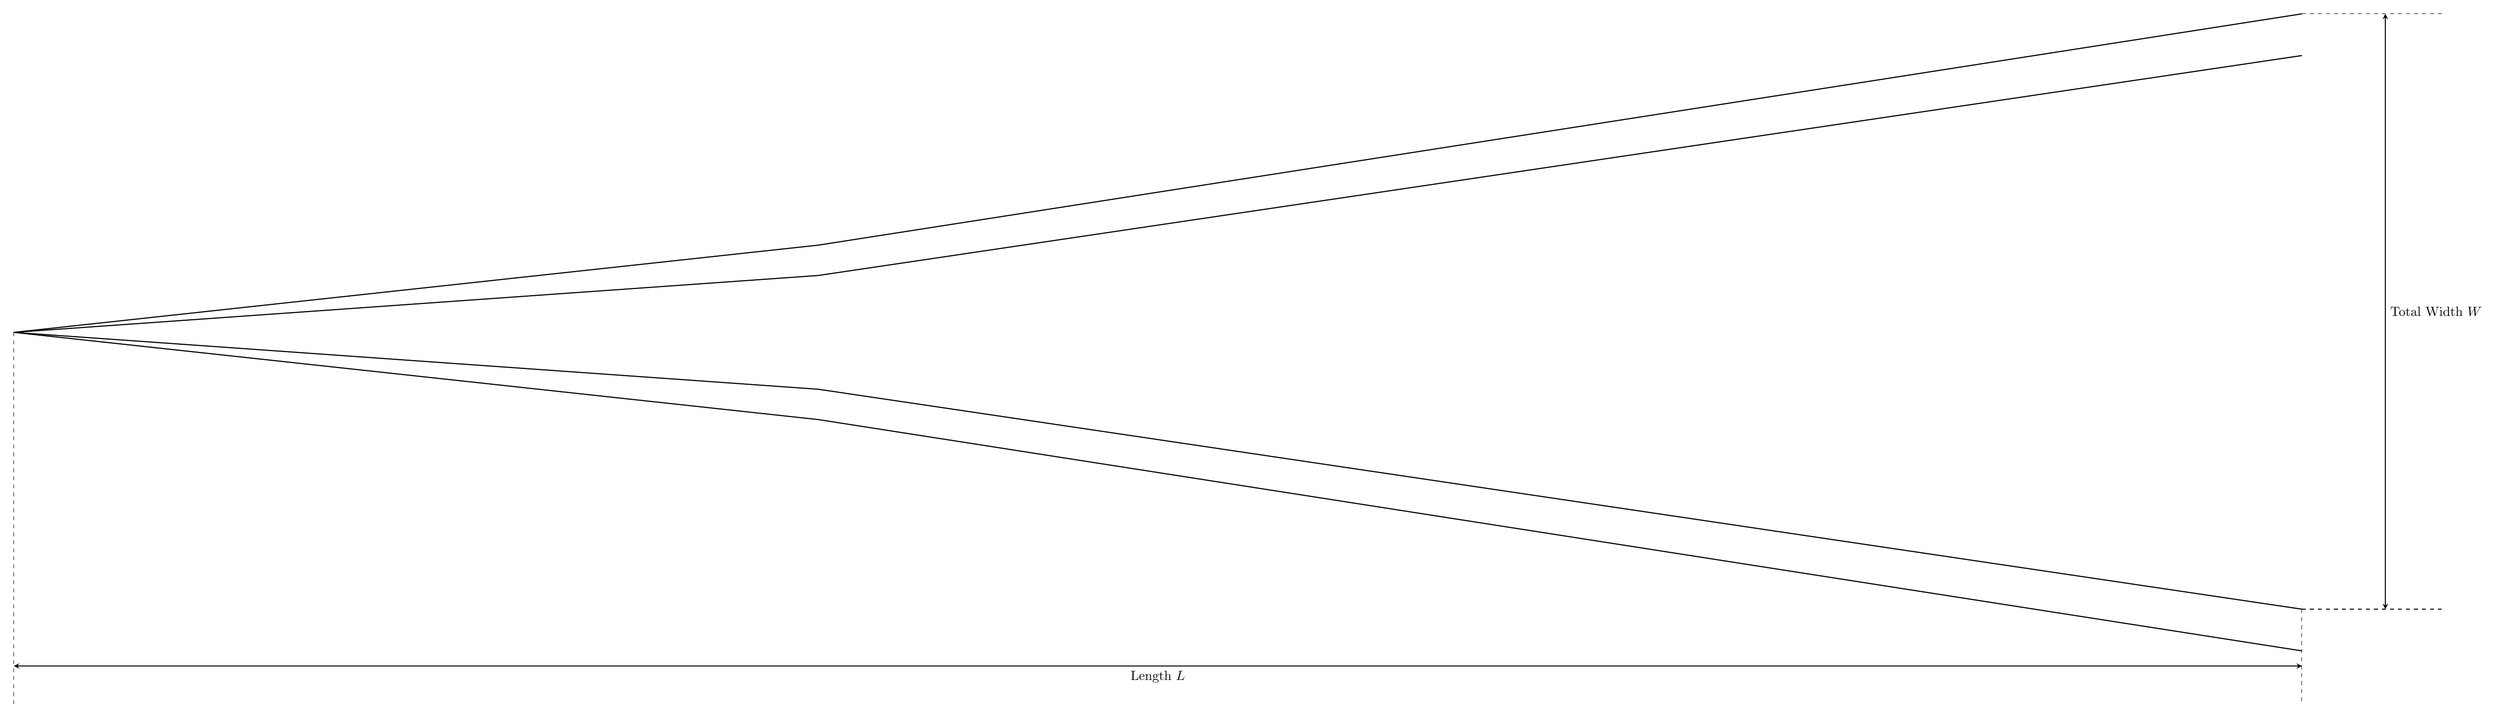
\begin{tikzpicture}[>=stealth, thick]

    % --- Coordinates ---
    \coordinate (A) at (0,14.8);
    \coordinate (B) at (21.2,13.3);
    \coordinate (C) at (21.2,16.3);
    \coordinate (D) at (60.3,7.5);
    \coordinate (E) at (60.3,22.1);
    \coordinate (F) at (21.2,17.1);
    \coordinate (G) at (21.2,12.5);
    \coordinate (H) at (60.3,6.4);
    \coordinate (I) at (60.3,23.2);

    % --- Draw Solid Wedges ---
    \draw (A) -- (B) -- (D);
    \draw (A) -- (C) -- (E);
    \draw (A) -- (F) -- (I);
    \draw (A) -- (G) -- (H);

    % --- Dimension Helpers (Extension Lines) ---
    % Vertical width dimension at x=60.3
    \draw[thin, dashed] (D) -- (64, 7.5);
    \draw[thin, dashed] (I) -- (64, 23.2);
    \draw[<->] (62.5, 7.5) -- (62.5, 23.2) node[midway, right] {Total Width $W$};

    % Length dimension (Horizontal)
    \draw[thin, dashed] (A) -- (0, 5);
    \draw[thin, dashed] (D) -- (60.3, 5);
    \draw[<->] (0, 6) -- (60.3, 6) node[midway, below] {Length $L$};

\end{tikzpicture}
\end{document}